
In this section, I present the results of applying the classification methods described above.

%Political scientists have thus far focused on sophisticated lobbying efforts. However, as 
\paragraph{Data.}
In his case-study of several rules, \citet{Cuellar2005} finds that ``contrary to conventional wisdom, comments from the lay public make up the vast majority of total comments about some regulations. This shows at least some potential demand among the mass public for a seat at the table in the regulatory process.'' 
With over 70 million comments on over 300,000 proposed rules, I am able to offer a much more systematic analysis. 

\paragraph{Most comments result from mass-comment campaigns.}
Figure \ref{fig:comments-mass} shows all comments posted on regulations.gov over time by whether they are exact copies of another comment or not. This highly restrictive definition of what counts as mass engagement captures comments that were certainly mobilized by a campaign. As \ref{fig:comments-mass} shows the vast majority of comments are mobilized by mass commenting campaigns. In other words, most comments are from ordinary people.

\begin{figure}[h!]
    \centering
        \caption{Unique vs Form-letter Comments Posted to Regulations.gov 2006-2018}
    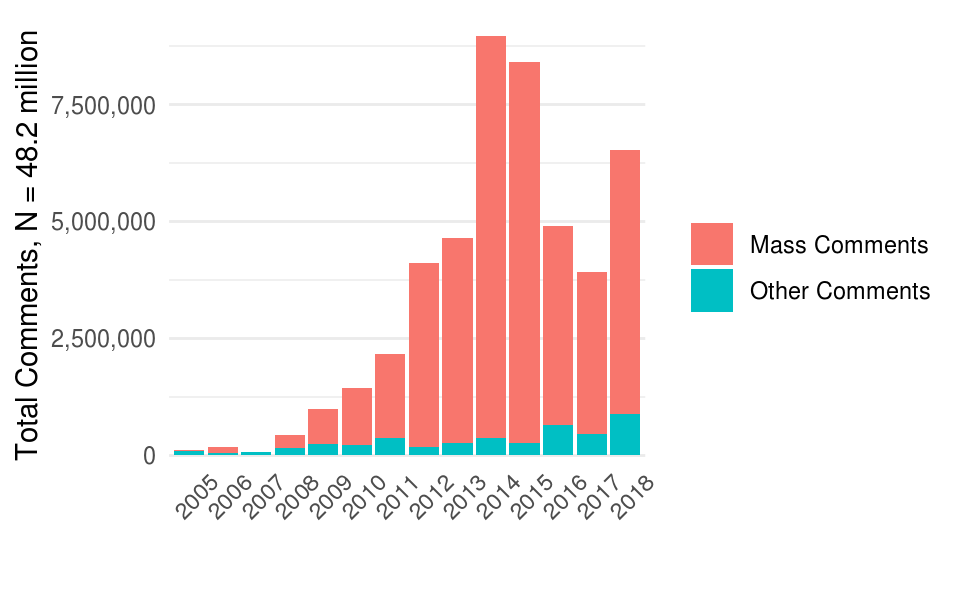
\includegraphics[height =2in]{Figs/comments-mass-vs-unique-1.png}
    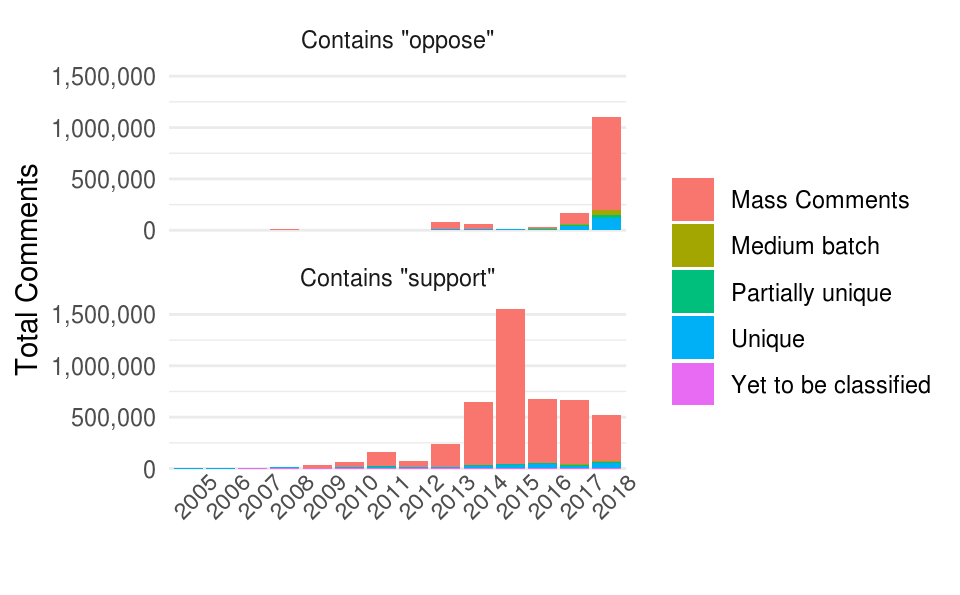
\includegraphics[height =2in]{Figs/comments-mass-support-vs-oppose-1.png}

    \label{fig:comments-mass}
\end{figure}

The right pane of \ref{fig:comments-mass} shows results from a sample of several million comments for which I have digitized texts. Many of these comments appear to support proposed agency rules, as was the case with both the do not call and mercury rule examples. A rough measure of support (whether the comment text includes `` support '' or `` oppose '') shows that many more comments mention support, until 2018, when there is a fairly dramatic reversal in the share of comments mentioning `` support '' compared to those mentioning ` `oppose '' (figure \ref{fig:comments-mass}). This may be a function of the changing regulatory agenda due to the change in presidential administration. 



\paragraph{Most comments occur on a small number of salient rules.} Approximately a third of public comments posted to regulations.gov were received on just ten dockets.


\begin{figure}
    \centering
    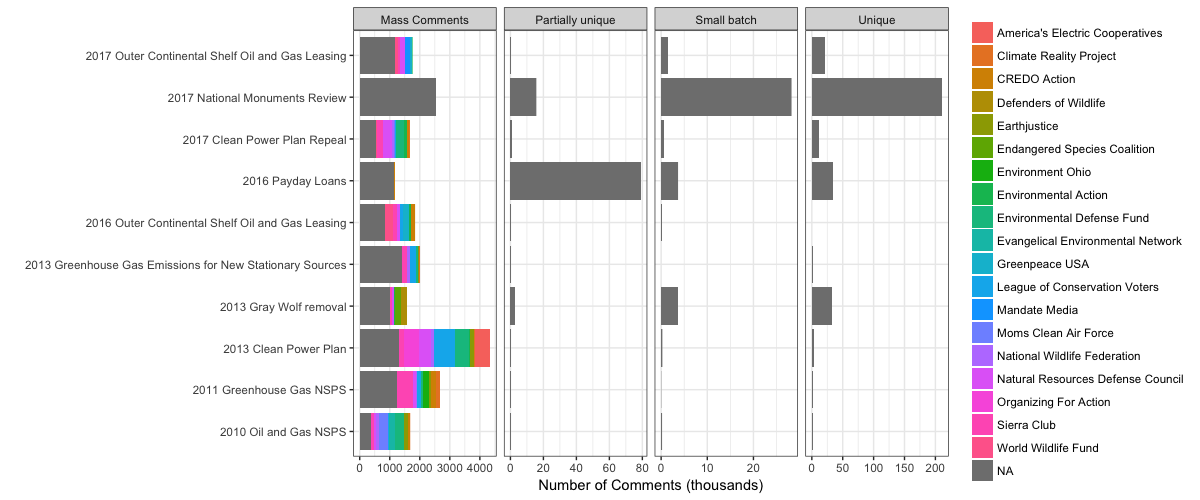
\includegraphics[width = 6in]{Figs/topdockets.png}
    \caption{Top 10 Dockets Receiving the Most Comments on regulations.gov and the 20 Mobilizers}
    \label{fig:topdockets}
\end{figure}


\paragraph{A coalition of public-interest organizations mobilize most comments.} As figures \ref{fig:topdockets}% and \ref{fig:toporgs} 
show, the most prolific mobilizers are environmental groups. In part, this is because the Environmental Protection Agency produces a large share of substantive rules posted to regulations.gov. However, it is notable that, on the top ten dockets, 19 of the top 20 mobilizers generally lobby together. America's Energy Cooperatives, an industry association, stands out as the lone mobilizer on behalf of material interest for its members. Notably, it only mobilized significantly on the Clean Power Plan. 